% figure1_pair_vpipe.tex — (a) pikv workflow + (b) vertical RepairKV pipe.
% Three stacked bands: GPU active (top), RepairKV pipe (middle, with signal
% entering from the left), Host pool (bottom). Two short vertical arrows
% carry K teal chips up through the pipe.  No curved arrows, no GPU-row
% overlap, naturally compact.
% Shared preamble for standalone Figure 1 variants.
\documentclass[border=8pt,tikz]{standalone}
\usepackage{amsmath}
\usepackage{amssymb}
\usepackage{tikz}
\usetikzlibrary{arrows.meta,positioning,calc,fit,shapes.geometric,backgrounds}
\usepackage{xcolor}
\usepackage[T1]{fontenc}
\usepackage{mathptmx}
\newcommand{\repairkv}{\textsc{RepairKV}}
\newcommand{\bbase}{\ensuremath{B_{\mathrm{base}}}}
\newcommand{\bmatch}{\ensuremath{B_{\mathrm{match}}}}

\begin{document}
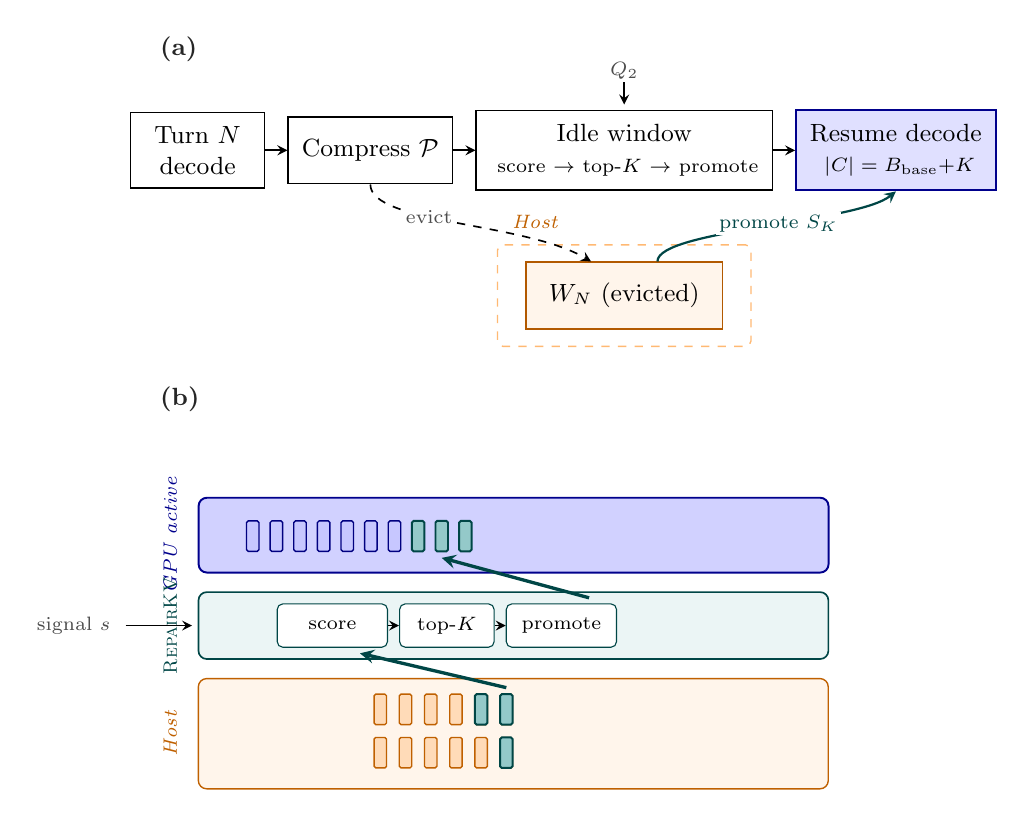
\begin{tikzpicture}[
  >=latex, line width=0.4pt,
  font=\small,
  % --- (a) pikv styles ---
  box/.style={draw=black, fill=white, line width=0.5pt,
              inner sep=5pt, align=center, minimum height=0.85cm},
  active/.style={box, fill=blue!12, draw=blue!55!black, line width=0.7pt},
  store/.style={box, fill=orange!8, draw=orange!70!black},
  arr/.style={->, line width=0.6pt, draw=black, >=stealth},
  promarr/.style={->, line width=0.8pt, draw=teal!55!black, >=stealth},
  arrlabel/.style={font=\scriptsize, text=black!70, fill=white, inner sep=1pt},
  groupbox/.style={draw=orange!55, dashed, line width=0.5pt, rounded corners=2pt},
  grouplabel/.style={font=\scriptsize\itshape, text=orange!75!black},
  panellabel/.style={font=\bfseries\small, text=black!85},
  % --- (b) banded layout styles ---
  bandgpu/.style={rounded corners=3pt, draw=blue!55!black, fill=blue!18,
                  line width=0.7pt, minimum height=0.95cm},
  bandhost/.style={rounded corners=3pt, draw=orange!75!black, fill=orange!8,
                   line width=0.5pt, minimum height=0.95cm},
  bandpipe/.style={rounded corners=3pt, draw=teal!55!black, fill=teal!8,
                   line width=0.6pt, minimum height=0.85cm},
  chip/.style={rounded corners=0.6pt, minimum width=4.5pt, minimum height=11pt,
               inner sep=0pt, line width=0.5pt},
  gpuchip/.style={chip, draw=blue!50!black, fill=blue!22},
  hostchip/.style={chip, draw=orange!75!black, fill=orange!28},
  promchip/.style={chip, draw=teal!55!black, fill=teal!42, line width=0.7pt},
  rowlabel/.style={font=\itshape\scriptsize},
  miniarr/.style={->, line width=0.7pt, draw=gray!55, >=stealth},
  bigpromarr/.style={->, line width=1.2pt, draw=teal!55!black, >=stealth},
  pipemod/.style={rounded corners=2pt, draw=teal!55!black, fill=white,
                  line width=0.4pt, inner sep=3pt, font=\scriptsize, align=center,
                  minimum height=0.55cm}
]
  % =================================================================
  % Panel (a) — pikv block diagram (top) — aligned at x=0.6
  % =================================================================
  \node[panellabel, anchor=south west] at (0, 4.4) {(a)};

  \node[box, minimum width=1.7cm] (dN) at (0.6, 3.4) {Turn $N$\\decode};
  \node[box, minimum width=1.6cm, right=8pt of dN] (cmp) {Compress~$\mathcal{P}$};
  \node[box, minimum width=2.5cm, right=8pt of cmp] (idle)
       {Idle window\\{\scriptsize{} score~$\to$~top-$K$~$\to$~promote}};
  \node[active, minimum width=1.9cm, right=8pt of idle] (resume)
       {Resume decode\\{\scriptsize{} $|C|=\bbase{+}K$}};

  \draw[arr] (dN) -- (cmp);
  \draw[arr] (cmp) -- (idle);
  \draw[arr] (idle) -- (resume);

  \draw[arr] ([yshift=10pt]idle.north) -- ([yshift=2pt]idle.north);
  \node[arrlabel, anchor=south] at ([yshift=10pt]idle.north) {$Q_2$};

  \node[store, minimum width=2.5cm, below=0.9cm of idle] (wn) {$W_N$ (evicted)};
  \node[groupbox, fit=(wn), inner xsep=10pt, inner ysep=6pt] (hgroup) {};
  \node[grouplabel, anchor=south west]
       at ([xshift=2pt, yshift=2pt]hgroup.north west) {Host};

  \draw[arr, dashed]
       (cmp.south) .. controls ([yshift=-0.5cm]cmp.south)
                              and ([yshift=0.5cm]wn.north west) ..
       ([xshift=-12pt]wn.north)
       node[arrlabel, pos=0.4] {evict};

  \draw[promarr]
       ([xshift=12pt]wn.north) .. controls ([xshift=12pt, yshift=0.4cm]wn.north)
                                          and ([xshift=-0.5cm, yshift=-0.4cm]resume.south) ..
       (resume.south)
       node[arrlabel, text=teal!55!black, pos=0.55] {promote~$S_K$};

  % =================================================================
  % Panel (b) — Vertical RepairKV pipe with chip lanes
  % =================================================================
  \node[panellabel, anchor=south west] at (0, -0.05) {(b)};

  % Three stacked bands: GPU (top), pipe (middle), Host (bottom).
  % Aligned to x=0.6, width 8.0cm. Vertical gaps prevent band/label overlap.
  \node[bandgpu, minimum width=8.0cm, minimum height=0.95cm,
        anchor=north west] (gpuband) at (0.6, -1.0) {};
  \node[bandpipe, minimum width=8.0cm, minimum height=0.85cm,
        anchor=north west] (piperow) at (0.6, -2.20) {};
  \node[bandhost, minimum width=8.0cm, minimum height=1.40cm,
        anchor=north west] (hostband) at (0.6, -3.30) {};

  % Tier labels (rotated, on left, italic, color-coded)
  \node[rowlabel, text=blue!55!black, anchor=south, rotate=90]
       at ([xshift=-4pt]gpuband.west) {GPU active};
  \node[rowlabel, text=teal!55!black, anchor=south, rotate=90]
       at ([xshift=-4pt]piperow.west) {\repairkv{}};
  \node[rowlabel, text=orange!75!black, anchor=south, rotate=90]
       at ([xshift=-4pt]hostband.west) {Host};

  % --- Pipe internals: three module pills inside the middle band ---
  \node[pipemod, minimum width=1.4cm, anchor=center]
       (mscore) at ([xshift=-2.3cm]piperow.center) {score};
  \node[pipemod, minimum width=1.2cm, right=4pt of mscore] (mselect)
       {top-$K$};
  \node[pipemod, minimum width=1.4cm, right=4pt of mselect] (mpromote)
       {promote};
  \draw[arr] (mscore.east)  -- (mselect.west);
  \draw[arr] (mselect.east) -- (mpromote.west);

  % --- Signal s entering pipe from the LEFT ---
  \draw[arr] ([xshift=-26pt]piperow.west) -- ([xshift=-2pt]piperow.west);
  \node[font=\scriptsize, text=black!70, anchor=east]
       at ([xshift=-28pt]piperow.west) {signal $s$};

  % --- Host chips: 12 in two sub-rows of 6 with 3 teal candidates ---
  % Band height 1.4cm, two rows centered at yshift -0.40 and -0.95 (clearance from top edge)
  \foreach \i in {1,...,6}{
    \foreach \r in {0,1}{
      \pgfmathsetmacro{\xh}{0.32*\i + 2.0}
      \pgfmathsetmacro{\yh}{-0.40 - 0.55*\r}
      \node[hostchip] at ([xshift=\xh cm, yshift=\yh cm]hostband.north west) {};
    }
  }
  % overlay teal candidates at right side: (5,0),(6,0),(6,1)
  \pgfmathsetmacro{\xPa}{0.32*5 + 2.0} \pgfmathsetmacro{\yPa}{-0.40}
  \pgfmathsetmacro{\xPb}{0.32*6 + 2.0} \pgfmathsetmacro{\yPb}{-0.40}
  \pgfmathsetmacro{\xPc}{0.32*6 + 2.0} \pgfmathsetmacro{\yPc}{-0.40 - 0.55}
  \node[promchip] (chostA) at ([xshift=\xPa cm, yshift=\yPa cm]hostband.north west) {};
  \node[promchip] (chostB) at ([xshift=\xPb cm, yshift=\yPb cm]hostband.north west) {};
  \node[promchip] (chostC) at ([xshift=\xPc cm, yshift=\yPc cm]hostband.north west) {};

  % --- GPU chips: 7 blue + 3 teal (the promoted ones, on right end) ---
  \foreach \i in {1,...,7}{
    \pgfmathsetmacro{\xc}{0.30*\i + 0.40}
    \node[gpuchip] at ([xshift=\xc cm, yshift=-0.5cm]gpuband.north west) {};
  }
  \foreach \i in {1,2,3}{
    \pgfmathsetmacro{\xs}{0.30*7 + 0.30*\i + 0.40}
    \node[promchip] (cgpuA\i) at ([xshift=\xs cm, yshift=-0.5cm]gpuband.north west) {};
  }

  % --- Two short vertical arrows: host -> pipe and pipe -> GPU ---
  % Up arrow from host candidates to mscore (entry into pipe)
  \draw[bigpromarr] ([yshift=2pt]chostB.north)
                    -- ([yshift=-2pt, xshift=10pt]mscore.south);
  % Up arrow from mpromote to GPU teal chips
  \draw[bigpromarr] ([yshift=2pt, xshift=10pt]mpromote.north)
                    -- ([yshift=-2pt]cgpuA2.south);
\end{tikzpicture}
\end{document}
